\section{Compact Torus Injector}
\begin{frame} {Central Fuelling of Tokamak}
    Central fuelling can:
    \begin{itemize}
        \item control plasma density and pressure profiles.
        \item make plasma to achieve high fuel burn-up rate and low tritium recycling.
        \item improve tokamak confinement.
    \end{itemize}

    However, conventional fuelling technologies (peripheral gas admission, and frozen pellet injection) have drawbacks:
    \begin{itemize}
        \item relatively low pellet speed prevents the direct fuel deposition beyond the separatrix in reactor-grade tokamak such as ITER.
        \item Energetic neutral beam injection is economically inefficient.
    \end{itemize}
\end{frame}

\begin{frame} {Compact Torus Injection}
    New injection technology, CT injection has some benefits:
    \begin{itemize}
        \item CT can be accelerated to hundreds of kilometers per second.
        \item Tangential CT injection may transfer CT momentum to tokamak plasma to induce and sustain toroidal rotation, good for stabilizing the locked mode and resistive wall mode.
        \item It is observed that tangential CT injection into STOR-M tokamak induces H-mode discharges.
    \end{itemize}
\end{frame}

\begin{frame} {Tangential Compact Torus Injection Setup}
    \begin{figure}
        \centering
        \begin{subfigure}{0.6\textwidth}
            \centering
            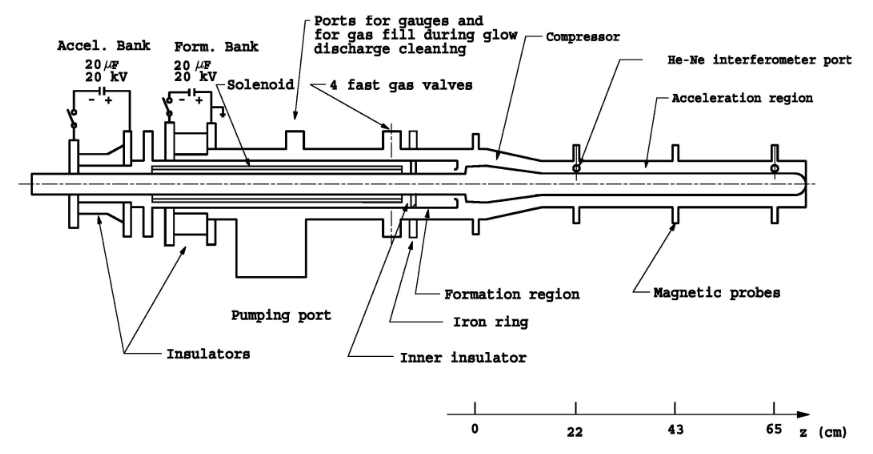
\includegraphics[width=\textwidth]{figures/uscti.png}
            \caption{Schematic diagram of USCTI. \cite{xiao_2004_improved}}
            \label{fig:uscti}
        \end{subfigure}%
        \begin{subfigure}{0.4\textwidth}
            \centering
            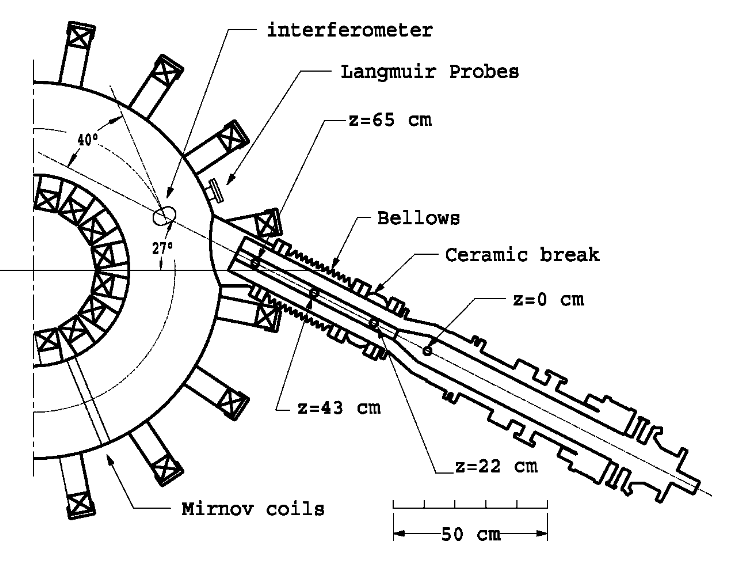
\includegraphics[width=\textwidth]{figures/tangential-cti-setup.png}
            \caption{Arrangement of CT injection experiments on the STOR-M tokamak. \cite{xiao_2004_improved}}
            \label{fig:tangential-cti-setup}
        \end{subfigure}
    \end{figure}

    \tiny \cite{xiao_2004_improved} C.Xiao, A. Hirose, and S.Sen. \textit{Improved confinement induced by tangential injection of compact torus into the saskatchewan torus-modified (stor-m) tokamak.}
\end{frame}